
% !TEX root = ../../phdthesis_tawatr.tex 
\renewcommand{\thisdir}{_content/htr_test}
\renewcommand{\figdir}{\thisdir/_fig}
\section{Examining the near-surface small-scale heterogeneity model}


\blueb{Introductory paragraph}
\begin{itemize}
	\item In the previous sections, we simulated the galvanic distortion with the random galvanic distortion parameters -- site gain, twist, shear and splitting parameters.
	\item In this section, we used the near-surface small-scale heterogeneity to represent the galvanic distortion effect in order to imitate the situation illustrated in Figure \ref{fig:galvanic_distortion_model}, which we may face in reality.
	\item The model of small-scale heterogeneity (Figure \ref{fig:htr_model}) was added to our 3D model (Figure \ref{fig:model3d_setting}) at the near-surface layer.
	The distribution of the resistivity of the small-scale heterogeniety model is assumed to be the normal distribution with the SD of XX and bounded within $(-XXX,XXX)$ in logarithmic scale (Figure \ref{fig:XXX}). The layer of heterogeneity was extended from the surface to XXX m depth. The MT array configuration remains the same as used in the 3D example (Figure \ref{fig:model3d_setting}).
	\item The models of the regional mean 1D conductivity profile from the average det and ssq impedances were shown in comparison with the 3D example without the near-surface heterogeneity layer. Also, the implication of  local and regional distortion indicators and the apparent gains was presented.
\end{itemize}

\blueb{Show the plots of results. Describe it and discussion.}
\begin{itemize}
	\item Showing the example of det and ssq from one stations probably the same station as in 3D example.
	\item Showing the det and ssq impedances from the whole clusters
	\item Showing the average det and ssq impedances from this model in comparison with the results from the model without the near-surface layer.
	\item Showing the local and regional distortion indicators.
	\item Showing the apparent gains.
\end{itemize}

\begin{figure}
	\centering
	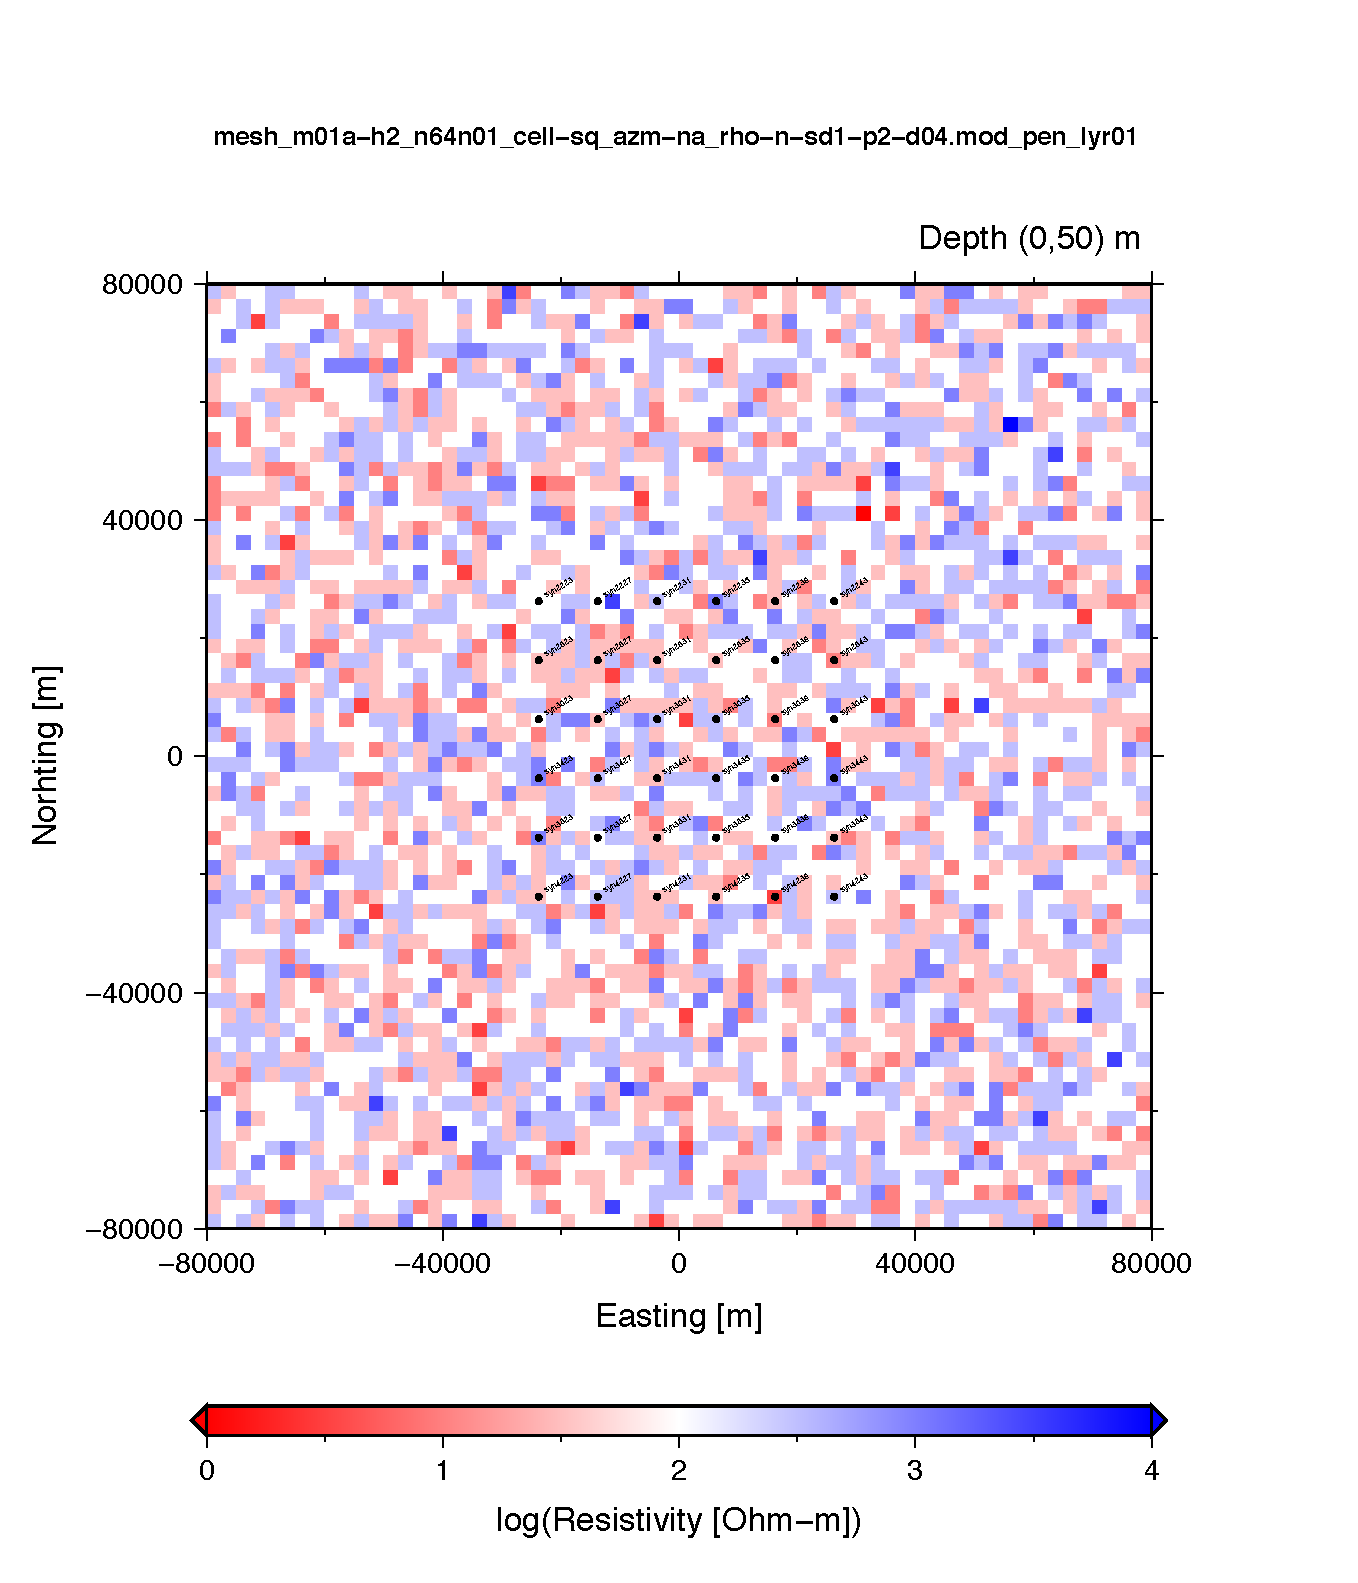
\includegraphics[scale=\plotdindmeanscale]{\figdir/htr_model.pdf}
	\caption{Example of the heterogeneity model. (Just an example) Here the heterogeneity size is 2.5 km x 2.5 km}
	\label{fig:htr_model}	
\end{figure}
